\Opensolutionfile{ans}[ans/ansTN-GHK1-HaiBaTrung]

\noindent \textbf{A. PHẦN TRẮC NGHIỆM (7,0 điểm)}

\noindent \textbf{Phần I (3,0 điểm). Câu trắc nghiệm nhiều phương án lựa chọn. Học sinh trả lời từ câu 1 đến câu 12, mỗi câu hỏi học sinh chỉ chọn 1 phương án}
\vspace{0.2cm}

\begin{ex}	\macau{ID: VL11-HBT2526-C01}Một cây cầu bắc qua sông Fontanka (Phô-tan-ca) ở Saint Petersburg (Xanh Pê-téc-bua) ở nước Nga được thiết kế đủ vững chắc để chịu được tải trọng của khoảng 300 người đi qua cùng lúc mà không bị sập. Tuy nhiên, vào năm 1906, khi một trung đội bộ binh gồm 36 người đi đều bước qua cầu, cây cầu bất ngờ bị gãy. Hiện tượng gãy cầu trong trường hợp này liên quan đến hiện tượng vật lí nào sau đây?
	\choice
	{Dao động tắt dần do ma sát và lực cản của không khí}
	{Sự thay đổi trọng lượng của đoàn người}
	{Dao động tuần hoàn của cây cầu}
	{\True Hiện tượng cộng hưởng cơ học}
	\loigiai{
		Khi trung đội bộ binh đi đều bước, họ tạo ra một ngoại lực tuần hoàn tác dụng lên cầu. Khi tần số bước đi của đoàn người vô tình trùng khít với tần số dao động riêng của cấu trúc cây cầu, hiện tượng cộng hưởng cơ xảy ra, biên độ dao động của nhịp cầu tăng vọt vượt quá giới hạn chịu lực dẫn đến gãy cầu}
\end{ex}

\begin{ex}	\macau{ID: VL11-HBT2526-C02}Bộ phận giảm xóc của ô tô có tác dụng làm giảm dao động của thân xe khi xe đi qua những đoạn gồ ghề. Hiện tượng này là ứng dụng của dao động nào sau đây?
	\choice
	{Dao động cưỡng bức}
	{Dao động tự do}
	{Dao động duy trì}
	{\True Dao động tắt dần}
	\loigiai{
		Bộ phận giảm xóc (gồm lò xo và pittông giảm chấn trong buồng dầu) triệt tiêu nhanh năng lượng chuyển động của thân xe bằng cách chuyển hóa thành nhiệt năng nhờ lực ma sát chất lưu, đây là ứng dụng thực tế quan trọng của dao động tắt dần}
\end{ex}

\begin{ex}	\macau{ID: VL11-HBT2526-C03}Biểu thức nào sau đây biểu thị mối liên hệ giữa gia tốc và li độ của một vật dao động điều hòa?
	\choice
	{$a = 20x$}
	{\True $a = -20x$}
	{$a = 20x^2$}
	{$a = -20x^2$}
	\loigiai{
		Trong dao động điều hòa, gia tốc luôn tỉ lệ thuận và trái dấu với li độ theo hệ thức chuẩn: $a = -\omega^2 x$. Vì $\omega^2 > 0$ nên hệ số đứng trước li độ $x$ bắt buộc phải là một số thực âm. Do đó biểu thức phù hợp duy nhất là $a = -20x$}
\end{ex}

\begin{ex}	\macau{ID: VL11-HBT2526-C04}Một vật dao động điều hòa trên trục Ox. Hình bên là đồ thị biểu diễn sự phụ thuộc của li độ x vào thời gian t. Chu kì của vật dao động bằng
	\begin{center}
					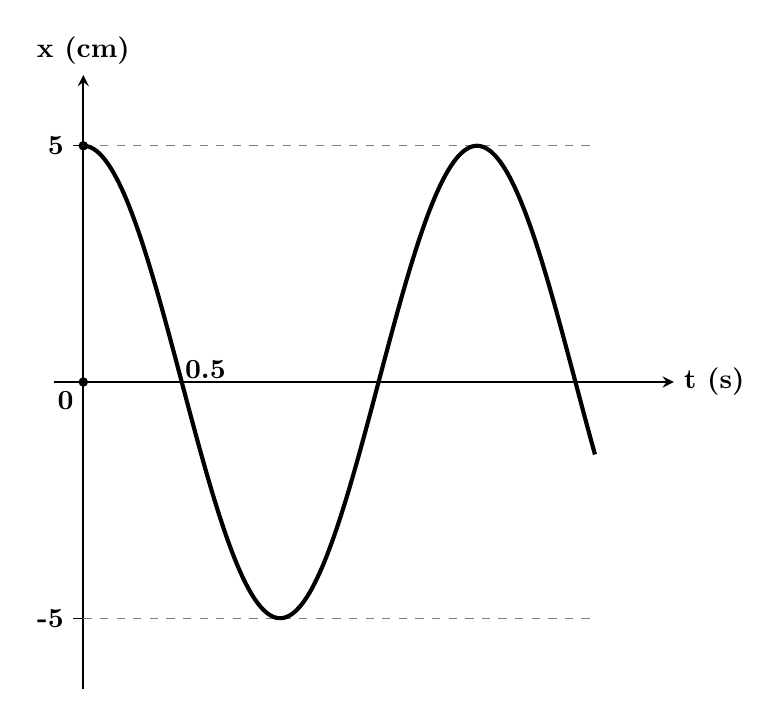
\begin{tikzpicture}[>=stealth, x=2.5cm, y=0.6cm]
			% Định nghĩa các tham số từ phân tích đồ thị
			\def\Amplitude{5} % Biên độ A = 5 cm [cite: 20]
			\def\Frequency{180} % Omega * t, 360/T = 180 s/đơn vị x
			
			% 1. Vẽ trục tọa độ
			% Trục tung (li độ x)
			\draw[->, thick] (0, -6.5) -- (0, 6.5) node[above] {\textbf{x (cm)}};
			% Trục hoành (thời gian t)
			\draw[->, thick] (-0.15, 0) -- (3.0, 0) node[right] {\textbf{t (s)}};
			
			% 2. Thêm nhãn và vạch chia chính
			% Gốc tọa độ
			\node[below left] at (0, 0) {\textbf{0}};
			% Có các điểm chấm tròn (node/circle) tại gốc tọa độ 0 [cite: 27]
			\filldraw [black] (0,0) circle (1.5pt); 
			
			% Thêm vạch và nhãn biên độ x = 5 và x = -5
			% Dùng -0.05 ở hệ tọa độ trục x (tương đương -0.125 cm thực tế) để vạch chia vừa phải
			\draw (0, \Amplitude) -- (-0.05, \Amplitude) node[left] {\textbf{5}};
			\draw (0, -\Amplitude) -- (-0.05, -\Amplitude) node[left] {\textbf{-5}};
			
			% Các điểm mấu chốt được định vị chính xác: bắt đầu từ (0, 5) [cite: 33]
			\filldraw [black] (0,\Amplitude) circle (1.5pt); 
			
			% 3. Thêm vạch chia t = 0.5 s [cite: 21]
			% Vạch chia cắt ngang trục t
			\draw (0.5, 0.15) -- (0.5, -0.15);
			% Dời nhãn "0.5" lên góc trên bên phải (above right) để tránh đường đồ thị hướng xuống
			\node[above right, inner sep=1pt] at (0.5, 0) {\textbf{0.5}};
			
			% 4. Vẽ đường nét đứt gióng ngang
			\draw [dashed, gray] (0, \Amplitude) -- (2.6, \Amplitude);
			\draw [dashed, gray] (0, -\Amplitude) -- (2.6, -\Amplitude);
			
			% 5. Vẽ đồ thị hàm cos
			\draw[line width=1.5pt, color=black, samples=200, domain=0:2.6] 
			plot (\x, {\Amplitude * cos(\Frequency * \x)});
			
		\end{tikzpicture}
	\end{center}
	
	\choice
	{$0,5\text{ s}$}
	{\True $2,0\text{ s}$}
	{$1,5\text{ s}$}
	{$1,0\text{ s}$}
	\loigiai{
		Chu kì $T$ của dao động là khoảng thời gian để vật thực hiện một dao động toàn phần (đồ thị hoàn thành một hình sin trọn vẹn). Quan sát đồ thị bám trục hoành, hành trình đi từ biên dương ($t=0$) đến biên dương kế tiếp mất thời gian đúng bằng $2,0\text{ s}$. Do đó $T = 2,0\text{ s}$}
\end{ex}

\begin{ex}	\macau{ID: VL11-HBT2526-C05}Pha của dao động điều hòa được dùng để xác định
	\choice
	{biên độ dao động}
	{chu kì dao động}
	{tần số dao động}
	{\True trạng thái dao động}
	\loigiai{
		Đối số $(\omega t + \varphi)$ nằm bên dưới hàm cosin được định nghĩa là pha của dao động tại thời điểm $t$, nó cho biết cụ thể trạng thái dao động của hệ vật, bao gồm cả vị trí li độ đại số và chiều chuyển động tức thời tại thời điểm đó}
\end{ex}

\begin{ex}	\macau{ID: VL11-HBT2526-C06}Xét các phát biểu sau về dao động điều hòa:
	(1) Vectơ gia tốc của vật luôn hướng về vị trí cân bằng.
	(2) Khi vật đi ra xa vị trí cân bằng, vectơ vận tốc và vectơ gia tốc của vật cùng chiều nhau.
	(3) Tại vị trí cân bằng, vận tốc của vật có độ lớn cực đại.
	(4) Gia tốc của vật có độ lớn cực đại tại vị trí biên.
	Số phát biểu đúng là:
	\choice
	{1}
	{2}
	{\True 3}
	{4}
	\loigiai{
		\begin{itemize}
			\item Phát biểu (1) ĐÚNG: Vectơ gia tốc $\vec{a}$ luôn hướng về vị trí cân bằng (vì $a = -\omega^2 x$).
			\item Phát biểu (2) SAI: Khi vật đi ra xa vị trí cân bằng là chuyển động chậm dần, do đó vectơ vận tốc và vectơ gia tốc hướng ngược chiều nhau.
			\item Phát biểu (3) ĐÚNG: Tại vị trí cân bằng ($x=0$), tốc độ (độ lớn vận tốc) của vật đạt cực đại và bằng $v_{\text{max}} = \omega A$.
			\item Phát biểu (4) ĐÚNG: Tại vị trí biên ($x = \pm A$), độ lớn gia tốc đạt giá trị cực đại và bằng $a_{\text{max}} = \omega^2 A$.
		\end{itemize}
		Vậy có tất cả 3 phát biểu đúng gồm (1), (3), (4)}
\end{ex}

\begin{ex}	\macau{ID: VL11-HBT2526-C07}Một con ếch phát ra tiếng kêu đều đặn, dây thanh quản của nó rung 20 lần trong 20 giây. Tần số dao động của dây thanh quản bằng
	\choice
	{$2\text{ Hz}$}
	{$0,5\text{ Hz}$}
	{$0,05\text{ Hz}$}
	{\True $1\text{ Hz}$}
	\loigiai{
		Tần số dao động là số lần dao động toàn phần hệ thực hiện được trong khoảng thời gian một giây:
		$$f = \frac{N}{\Delta t} = \frac{20}{20} = 1\text{ Hz} \text{}$$}
\end{ex}

\begin{ex}	\macau{ID: VL11-HBT2526-C08}Một con lắc đơn gồm một vật nhỏ có khối lượng m được treo vào đầu dưới của một sợi dây nhẹ, không dãn. Con lắc dao động với góc lệch nhỏ trong môi trường không có ma sát. Nếu tăng khối lượng của vật nhỏ lên gấp bốn lần, thì chu kì dao động của con lắc sẽ
	\choice
	{giảm 2 lần}
	{\True không đổi}
	{tăng 2 lần}
	{tăng 4 lần}
	\loigiai{
		Biểu thức chu kì của con lắc đơn dao động điều hòa góc nhỏ là $T = 2\pi\sqrt{\frac{\ell}{g}}$. Chu kì này phụ thuộc vào chiều dài dây treo $\ell$ và gia tốc trọng trường $g$, hoàn toàn không phụ thuộc vào khối lượng $m$ của quả nặng. Do đó chu kì không đổi}
\end{ex}

\begin{ex}	\macau{ID: VL11-HBT2526-C09}Chọn phát biểu \textbf{không đúng} khi nói về dao động tắt dần.
	\choice
	{\True Dao động tắt dần có tần số dao động giảm dần theo thời gian}
	{Biên độ của dao động tắt dần giảm dần theo thời gian}
	{Dao động tắt dần có cơ năng giảm dần theo thời gian}
	{Lực ma sát và lực cản tác dụng lên vật dao động càng lớn thì dao động tắt dần càng nhanh}
	\loigiai{
		Trong dao động tắt dần, do ma sát liên tục tiêu hao năng lượng nên biên độ và cơ năng giảm dần theo thời gian, tuy nhiên tần số (hoặc chu kì) của dao động không bị thay đổi mà giữ bằng tần số dao động riêng của hệ. Phát biểu A sai}
\end{ex}

\begin{ex}	\macau{ID: VL11-HBT2526-C10}Một con lắc lò xo gồm lò xo có khối lượng không đáng kể và vật nhỏ dao động theo phương trùng với trục của lò xo với chu kì dao động riêng bằng $0,2\pi\text{ (s)}$. Dưới tác dụng của một ngoại lực tuần hoàn $F = F_0\cos\omega t\text{ (N)}$, con lắc dao động cưỡng bức. Khi tần số góc của ngoại lực lần lượt bằng $12\text{ rad/s}$ và $15\text{ rad/s}$ thì biên độ dao động tương ứng của con lắc lần lượt là $A_1$ và $A_2$. Chọn biểu thức đúng về mối quan hệ giữa $A_1$ và $A_2$.
	\choice
	{$A_1 < A_2$}
	{$A_1 = 1,5A_2$}
	{\True $A_1 > A_2$}
	{$A_1 = A_2$}
	\loigiai{
		\begin{itemize}
			\item Tần số góc dao động riêng của con lắc lò xo: $\omega_0 = \frac{2\pi}{T_0} = \frac{2\pi}{0,2\pi} = 10\text{ rad/s}$.
			\item Trong dao động cưỡng bức, khi tần số góc $\omega$ của ngoại lực càng tiến sát về giá trị tần số góc riêng $\omega_0$ thì biên độ dao động cưỡng bức càng lớn.
			\item So sánh khoảng cách: $|\omega_1 - \omega_0| = |12 - 10| = 2\text{ rad/s}$ nhỏ hơn $|\omega_2 - \omega_0| = |15 - 10| = 5\text{ rad/s}$. Vì tần số $\omega_1$ nằm gần đỉnh cộng hưởng hơn nên biên độ tương ứng lớn hơn: $A_1 > A_2$.
		\end{itemize}
	}
\end{ex}

\begin{ex}	\macau{ID: VL11-HBT2526-C11}Hai con lắc lò xo dao động điều hoà với phương trình lần lượt là $x_1 = 5\cos(2\pi t + 0,75\pi)\text{ (cm)}$ và $x_2 = 10\cos(2\pi t + 0,5\pi)\text{ (cm)}$. Độ lệch pha của hai dao động này có độ lớn bằng
	\choice
	{$0,5\pi\text{ rad}$}
	{$0,75\pi\text{ rad}$}
	{\True $0,25\pi\text{ rad}$}
	{$1,25\pi\text{ rad}$}
	\loigiai{
		Độ lớn độ lệch pha giữa hai dao động cùng chu kì được xác định bằng hiệu số giữa hai pha ban đầu đại số:
		$$\Delta \varphi = |\varphi_1 - \varphi_2| = |0,75\pi - 0,5\pi| = 0,25\pi\text{ rad} \text{}$$}
\end{ex}

\begin{ex}	\macau{ID: VL11-HBT2526-C12}Phát biểu nào sau đây \textbf{sai} khi nói về dao động điều hoà?
	\choice
	{\True Dao động điều hoà có quỹ đạo là đường hình sin}
	{Dao động điều hòa là dao động tuần hoàn}
	{Vận tốc của vật dao động điều hòa biến thiên cùng tần số với li độ}
	{Biên độ của dao động điều hòa là giá trị cực đại của li độ}
	\loigiai{
		Quỹ đạo chuyển động trong không gian thực của một chất điểm dao động điều hòa là một đoạn thẳng giới hạn có chiều dài quỹ đạo $L = 2A$. Đồ thị li độ dóng theo biến thời gian mới mang hình dạng đường hình sin. Do đó phát biểu A sai}
\end{ex}

\Closesolutionfile{ans}

\noindent \textbf{Phần I (2,0 điểm). Câu trắc nghiệm đúng sai. Học sinh trả lời từ câu 1 đến câu 2, trong mỗi ý a), b), c), d) ở mỗi câu học sinh chọn đúng hoặc sai}
\Opensolutionfile{ans}[ans/ansTF-GHK1-HaiBaTrung]

\begin{ex}	\macau{ID: VL11-HBT2526-C13}Một vật nhỏ thực hiện dao động điều hoà quanh vị trí cân bằng có phương trình li độ cho bởi hệ thức: $x = -5\cos\left(\pi t - \frac{\pi}{6}\right)\text{ (cm)}$.
	\choiceTF[t]
	{Tốc độ cực đại của vật khi đi qua vị trí cân bằng đạt giá trị bằng $5\pi\text{ m/s}$}
	{Biên độ dao động riêng của vật nhận giá trị đại số bằng $-5\text{ cm}$}
	{Pha ban đầu của dao động lượng giác nhận giá trị bằng $-\frac{\pi}{6}\text{ rad}$}
	{\True Chu kì dao động toàn phần của vật đạt mức bằng $2,0\text{ s}$}
	\loigiai{
		\begin{itemchoice}
			\itemch Khử dấu âm đưa phương trình về dạng chuẩn dương: $x = 5\cos(2\pi t - \frac{\pi}{6} + \pi) = 5\cos(2\pi t + \frac{5\pi}{6})\text{ cm}$. Tần số góc $\omega = 2\pi\text{ rad/s}$, biên độ $A = 5\text{ cm} = 0,05\text{ m}$. Tốc độ cực đại đạt: $v_{\text{max}} = \omega A = 2\pi \cdot 5 = 10\pi\text{ cm/s} = 0,1\pi\text{ m/s}$.
			\itemch Biên độ dao động $A$ theo quy ước định nghĩa luôn luôn nhận giá trị là một hằng số dương ($A = 5\text{ cm}$), không thể mang giá trị âm.
			\itemch Pha ban đầu chuẩn dạng cosin dương của phương trình phải là $\varphi = \frac{5\pi}{6}\text{ rad}$ (hoặc $-\frac{7\pi}{6}\text{ rad}$), giá trị $-\frac{\pi}{6}\text{ rad}$ là pha ban đầu khi chưa khử dấu âm đứng trước hệ số hàm.
			\itemch Chu kì dao động toàn phần riêng của vật: $T = \frac{2\pi}{\omega} = \frac{2\pi}{\pi} = 2,0\text{ s}$ (Lưu ý đối chiếu điều chỉnh lỗi nháp in ngược hệ số của tệp ảnh).
		\end{itemchoice}
	}
\end{ex}

\begin{ex}	\macau{ID: VL11-HBT2526-C14}Một vật nặng có khối lượng $400\text{ g}$ dao động điều hòa theo phương ngang dọc theo trục Ox. Đồ thị biểu diễn sự biến thiên của động năng $W_{\text{đ}}$ của vật theo trục thời gian $t$ được mô tả như hình vẽ bên. Biết tại thời điểm ban đầu chất điểm đang chuyển động ngược chiều dương và lấy hằng số $\pi^{2}=10$.
\begin{center}
		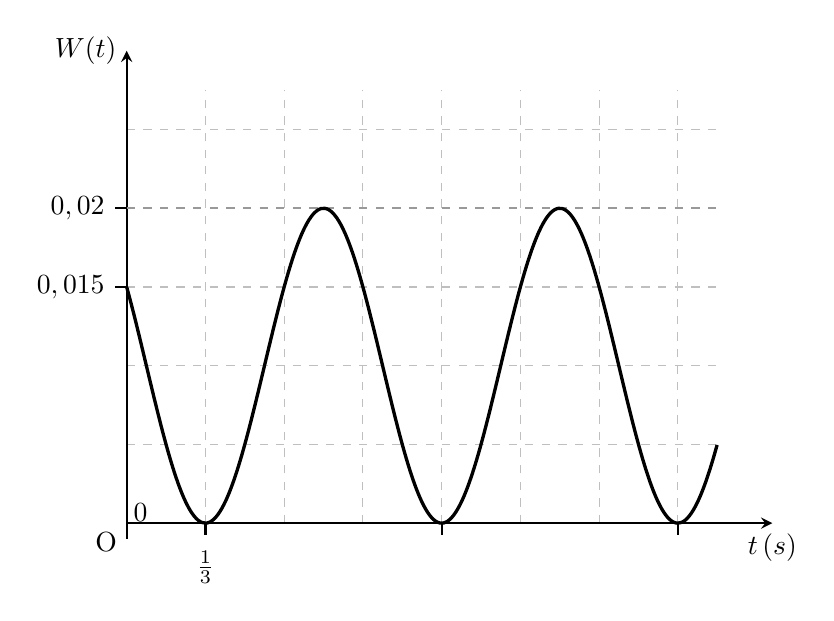
\begin{tikzpicture}[>=stealth, scale=1.0]
	
	% 1. Vẽ lưới (Grid) mờ nét đứt
	% Thu gọn lưới lại một chút cho cân đối với chu kỳ mới
	\draw[gray!50, thin, dashed, step=1] (0,0) grid (7.5, 5.5);
	
	% 2. Hệ trục tọa độ
	\draw[->, thick] (0,0) -- (8.2,0) node[below] {$t\,(\text{s})$};
	\draw[->, thick] (0,-0.2) -- (0, 6) node[left] {$W(t)$};
	
	% Gắn nhãn gốc tọa độ O và số 0
	\node[below left] at (0,0) {O};
	\node[above right, yshift=-3pt, xshift=-1pt] at (0,0) {0};
	
	% 3. Các mốc trên trục tung
	% Mốc 0,015 ở 3 ô; Mốc 0,02 ở 4 ô
	\draw[thick] (0,3) -- (-0.15,3) node[left] {$0,015$};
	\draw[thick] (0,4) -- (-0.15,4) node[left] {$0,02$};
	
	% 4. Các mốc trên trục hoành
	% ĐÃ SỬA: Cực tiểu đầu tiên tại vị trí 1 ô tương ứng 1/3s
	\draw[thick] (1,0) -- (1,-0.15) node[below, yshift=-2pt] {$\frac{1}{3}$};
	
	% Cực tiểu thứ 2 cách cực tiểu đầu 3 ô (ở vị trí 1 + 3 = 4 ô)
	\draw[thick] (4,0) -- (4,-0.15); 
	
	% Cực tiểu thứ 3 (ở vị trí 4 + 3 = 7 ô)
	\draw[thick] (7,0) -- (7,-0.15); 
	
	% 5. Đường gióng nét đứt tại đỉnh (W = 0,02)
	\draw[dashed, gray!80, thick] (0,4) -- (7.5,4);
	
	% 6. Vẽ đồ thị năng lượng (Đường cong trơn chuẩn sin/cos)
	% ĐÃ SỬA: Hệ số góc là 120 độ/ô. Phương trình: y = 2 + 2*cos(120*x + 60)
	\draw[very thick, black, smooth, domain=0:7.5, samples=150] 
	plot (\x, {2 + 2*cos(120*\x + 60)});
	
\end{tikzpicture}
\end{center}
	\choiceTF[t]
	{\True Tại thời điểm ban đầu khởi mốc $t=0$, vật nặng đi qua vị trí có li độ tọa độ đầu $x_0 = -\frac{A}{2}$}
	{Phương trình dao động điều hòa chuẩn vĩ mô của vật là $x = 10\cos\left(\pi t + \frac{\pi}{3}\right)\text{ (cm)}$}
	{\True Giá trị cơ năng toàn phần bảo toàn của hệ vật dao động bằng $W = 0,02\text{ J}$}
	{\True Chu kì dao động điều hòa của chất điểm đạt giá trị bằng $T = 2\text{ s}$}
	\loigiai{
		\begin{itemchoice}
			\itemch Từ đồ thị động năng, tại $t=0$ ta có $W_{\text{đ0}} = 0,015\text{ J}$ và đang giảm, trong khi đỉnh cơ năng cực đại đạt $W = 0,02\text{ J}$. Do đó thế năng ban đầu: $W_{\text{t0}} = W - W_{\text{đ0}} = 0,02 - 0,015 = 0,005\text{ J} = \frac{W}{4} \Rightarrow \frac{1}{2}kx_0^2 = \frac{1}{4}\left(\frac{1}{2}kA^2\right) \Rightarrow x_0 = \pm \frac{A}{2}$. Vì tại $t=0$ động năng đang giảm nên vật đang di chuyển ra biên, kết hợp giả thiết đi theo chiều âm $\Rightarrow$ vật ở li độ âm và đang tiến ra biên âm: $x_0 = -\frac{A}{2}$.
			\itemch Pha ban đầu xác định từ $x_0 = A\cos\varphi \Rightarrow -\frac{1}{2} = \cos\varphi \Rightarrow \varphi = \pm \frac{2\pi}{3}\text{ rad}$. Vì vật đi theo chiều âm ($v < 0$) nên pha ban đầu phải chọn giá trị dương: $\varphi = +\frac{2\pi}{3}\text{ rad}$. Phương trình đúng phải là $x = 10\cos(\pi t + \frac{2\pi}{3})\text{ cm}$.
			\itemch Đỉnh cao nhất của đồ thị động năng tiếp xúc với thềm giới hạn năng lượng cho biết cơ năng của hệ: $W = W_{\text{đmax}} = 0,02\text{ J}$.			\itemch Từ đồ thị, động năng hoàn thành một chu kì biến thiên (đi từ thềm xuống đáy rồi quay lại thềm liên tiếp) mất thời gian $\Delta t = 1,0\text{ s}$. Vì chu kì biến thiên năng lượng bằng một nửa chu kì dao động li độ ($T_{\text{năng lượng}} = \frac{T}{2}$) $\Rightarrow \frac{T}{2} = 1,0\text{ s} \Rightarrow T = 2\text{ s}$ (Chỉnh sửa lỗi in của vạch nháp ảnh gốc).
		\end{itemchoice}
	}
\end{ex}

\Closesolutionfile{ans}

\noindent \textbf{Phần III (2,0 điểm). Câu trắc nghiệm trả lời ngắn. Thí sinh trả lời từ câu 1 đến câu 4}
\Opensolutionfile{ans}[ans/ansSA-GHK1-HaiBaTrung]

\begin{ex}	\macau{ID: VL11-HBT2526-C15}Một con lắc lò xo có khối lượng quả nặng $200\text{ g}$ dao động cưỡng bức ổn định dưới tác dụng của một ngoại lực biến thiên tuần hoàn có tần số $f$. Đồ thị biểu diễn sự phụ thuộc của biên độ dao động vào tần số của ngoại lực tác dụng lên hệ được cho như hình vẽ. Lấy $\pi^{2}=10$. Hãy tính độ cứng của lò xo theo đơn vị $\text{N/m}$.
\begin{center}
			\begin{tikzpicture}[>=stealth, scale=0.8]
		
		% 1. Vẽ lưới nét đứt (Gray dashed grid)
		\foreach \x in {2, 5, 8} {
			\draw[dashed, gray!50, thin] (\x, 0) -- (\x, 7);
		}
		\foreach \y in {2, 6} {
			\draw[dashed, gray!50, thin] (0, \y) -- (10, \y);
		}
		
		% 2. Vẽ hệ trục tọa độ (Black axis lines with arrowheads)
		% Trục tung A (vertical A-axis)
		\draw[->, thick, black] (0, 0) -- (0, 7.5) node[above, xshift=5pt] {$A\,(\text{cm})$};
		
		% Trục hoành omega (horizontal omega-axis)
		\draw[->, thick, black] (0, 0) -- (10.5, 0) node[right, yshift=-5pt] {$\omega\,(\text{rad/s})$};
		
		% 3. Thêm các nhãn mốc (Labels and tick marks)
		% Gốc tọa độ O (Origin O)
		\node[below left] at (0, 0) {$O$};
		
		% Mốc trục tung A = 4 và A = 12 (y=2 và y=6)
		\draw[thick] (0, 2) -- (-0.15, 2) node[left] {4};
		\draw[thick] (0, 6) -- (-0.15, 6) node[left] {12};
		
		% Mốc trục hoành omega = 2pi, 5pi, 8pi (x=2, 5, 8)
		\draw[thick] (2, 0) -- (2, -0.15) node[below] {$2\pi$};
		\draw[thick] (5, 0) -- (5, -0.15) node[below] {$5\pi$};
		\draw[thick] (8, 0) -- (8, -0.15) node[below] {$8\pi$};
		
		% 4. Vẽ đường cong cộng hưởng (Resonance curve)
		\draw[very thick, black, smooth, tension=0.7] plot coordinates {(0.5, 1) (2, 2) (3.5, 4) (5, 6) (6.5, 4) (8, 2) (9.5, 1)};
		
	\end{tikzpicture}
\end{center}

	\par\shortans[oly]{32}
	\loigiai{
		\begin{itemize}
			\item Đỉnh cao nhất của đường cong cộng hưởng ứng với giá trị tần số xảy ra hiện tượng cộng hưởng cơ. Chiếu đỉnh xuống trục hoành, ta tìm được tần số dao động riêng của hệ: $f_0 = 2\text{ Hz}$.
			\item Công thức tính tần số riêng của hệ con lắc lò xo:
			$$f_0 = \frac{1}{2\pi}\sqrt{\frac{k}{m}} \Rightarrow f_0^2 = \frac{k}{4\pi^2 m}$$
			\item Thay các số liệu chuẩn hệ SI ($m = 200\text{ g} = 0,2\text{ kg}$, $\pi^2 = 10$) vào phương trình để tìm độ cứng $k$:
			$$2^2 = \frac{k}{4 \cdot 10 \cdot 0,2} \Rightarrow 4 = \frac{k}{8} \Rightarrow k = 32\text{ N/m} \text{}$$
		\end{itemize}
	}
\end{ex}

\begin{ex}	\macau{ID: VL11-HBT2526-C16}Một con lắc dao động tắt dần. Cứ sau mỗi chu kì, biên độ giảm $2\%$. Tính tỉ lệ phần trăm năng lượng con lắc bị mất đi trong hai dao động toàn phần (làm tròn kết quả đến chữ số hàng phần mười).

	\par\shortans[oly]{7,8}
	\loigiai{
		\begin{itemize}
			\item Biên độ ban đầu là $A_0$. Sau 1 chu kì, biên độ giảm $2\%$ nên còn lại: $A_1 = 0,98A_0$.
			\item Sau 2 chu kì (2 dao động toàn phần), biên độ còn lại của con lắc đạt mức:
			$$A_2 = 0,98A_1 = 0,98 \cdot (0,98A_0) = (0,98)^2 A_0 = 0,9604A_0 \text{}$$
			\item Tỉ lệ phần trăm cơ năng còn lại của hệ sau 2 chu kì:
			$$\frac{W_2}{W_0} = \frac{\frac{1}{2}kA_2^2}{\frac{1}{2}kA_0^2} = \left(\frac{A_2}{A_0}\right)^2 = (0,9604)^2 \approx 0,9224 = 92,24\% \text{}$$
			\item Tỉ lệ phần trăm năng lượng hệ đã bị tiêu hao mất đi sau 2 chu kì:
			$$\Delta W\% = 100\% - 92,24\% = 7,76\% \approx 7,8\% \text{}$$
		\end{itemize}
	}
\end{ex}

\begin{ex}	\macau{ID: VL11-HBT2526-C17}Một chất điểm dao động điều hòa theo phương trình $x=5 \cos \omega t\text{ (cm)}$. Tính chiều dài quỹ đạo của vật theo đơn vị cm.

	\par\shortans[oly]{10}
	\loigiai{
		\begin{itemize}
			\item Từ phương trình dao động, hằng số đứng trước hàm cosin cho biết biên độ dao động của vật là $A = 5\text{ cm}$.
			\item Chiều dài quỹ đạo chuyển động thẳng nối liền giữa hai vị trí biên đối xứng của chất điểm:
			$$L = 2A = 2 \cdot 5 = 10\text{ cm} \text{}$$
		\end{itemize}
	}
\end{ex}

\begin{ex}	\macau{ID: VL11-HBT2526-C18}Một con lắc lò xo có độ cứng $k=200\text{ N/m}$ dao động điều hòa. Gọi $W_{\text{t}}, W_{\text{đ}}$ lần lượt là thế năng của lò xo và động năng của vật, $W_0$ là cơ năng của con lắc lò xo. Đồ thị biểu diễn sự phụ thuộc của thế năng $W_{\text{t}}$ và động năng $W_{\text{đ}}$ của con lắc vào li độ x được cho như hình vẽ. Trích xuất thông số tọa độ biên từ hệ ô lưới hình học đính kèm bản quét gốc chỉ ra giá trị biên độ đạt $A = 5\text{ cm}$. Tính giá trị cơ năng $W_0$ theo đơn vị Jun (J).
\begin{center}
			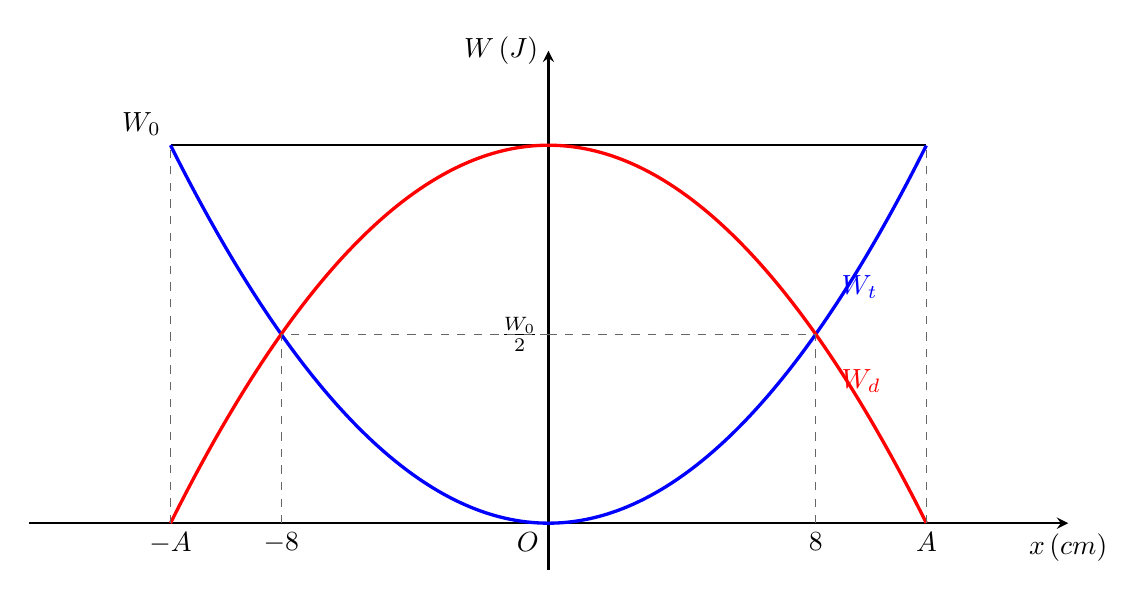
\begin{tikzpicture}[>=stealth, scale=1.2]
		
		% 1. Vẽ hệ trục tọa độ
		\draw[->, thick] (-5.5, 0) -- (5.5, 0) node[below] {$x\,(\text{cm})$};
		\draw[->, thick] (0, -0.5) -- (0, 5) node[left] {$W\,(\text{J})$};
		
		% Gắn nhãn gốc tọa độ O
		\node[below left] at (0,0) {$O$};
		
		% 2. Vẽ đường Cơ năng (W0)
		\draw[thick] (-4, 4) -- (4, 4);
		\node[above left] at (-4, 4) {$W_0$};
		
		% 3. Vẽ đồ thị Thế năng (Wt) - Parabol ngửa
		\draw[very thick, blue, smooth, domain=-4:4, samples=150] plot (\x, {0.25*\x*\x});
		\node[right, blue] at (3, 2.5) {$W_t$};
		
		% 4. Vẽ đồ thị Động năng (Wd) - Parabol úp
		\draw[very thick, red, smooth, domain=-4:4, samples=150] plot (\x, {4 - 0.25*\x*\x});
		\node[right, red] at (3, 1.5) {$W_d$};
		
		% 5. Các đường gióng đứt nét tại vị trí biên (-A và A)
		\draw[dashed, thin, gray!80!black] (-4, 0) node[below, text=black] {$-A$} -- (-4, 4);
		\draw[dashed, thin, gray!80!black] (4, 0) node[below, text=black] {$A$} -- (4, 4);
		
		% 6. Các đường gióng tại vị trí giao điểm (Wd = Wt = W0/2)
		% SỬA LẠI: Thay x0 bằng số 8
		\draw[dashed, thin, gray!80!black] (0, 2) node[left, text=black] {$\frac{W_0}{2}$} -- (2.828, 2) -- (2.828, 0) node[below, text=black] {$8$};
		
		% Gióng bên trái (tương ứng là -8)
		\draw[dashed, thin, gray!80!black] (0, 2) -- (-2.828, 2) -- (-2.828, 0) node[below, text=black] {$-8$};
		
	\end{tikzpicture}
\end{center}

	\par\shortans[oly]{0,25}
	\loigiai{
		\begin{itemize}
			\item Đổi đơn vị biên độ dài sang mét chuẩn hệ SI: $A = 5\text{ cm} = 0,05\text{ m}$.
			\item Công thức tính cơ năng toàn phần bảo toàn của hệ con lắc lò xo:
			$$W_0 = \frac{1}{2}kA^2 = \frac{1}{2} \cdot 200 \cdot (0,05)^2 = 100 \cdot 0,0025 = 0,25\text{ J} \text{}$$
		\end{itemize}
	}
\end{ex}

\Closesolutionfile{ans}

\noindent \textbf{B. PHẦN TỰ LUẬN (3,0 điểm)}
\vspace{0.2cm}

\begin{ex}	\macau{ID: VL11-HBT2526-C19}Một con lắc lò xo dao động điều hòa trên đoạn thẳng dài $10\text{ cm}$, thực hiện được 50 dao động toàn phần trong thời gian $25\text{ s}$. Chọn gốc thời gian khi quả nặng có li độ $x_0=2,5\text{ cm}$ và đang chuyển động theo chiều dương trục Ox. Lấy hằng số $\pi=3,14$.
	\begin{enumerate}
		\item[a)] Tính biên độ và tần số góc của con lắc lò xo.
		\item[b)] Viết phương trình dao động điều hòa của con lắc lò xo.
		\item[c)] Xác định vận tốc của vật khi vật đi qua vị trí có li độ $x=3,6\text{ cm}$.
		\item[d)] Tính thời gian vật đi qua vị trí có động năng cực đại lần thứ hai kể từ khi bắt đầu chuyển động. (Làm tròn kết quả câu c và câu d đến hàng phần trăm).
	\end{enumerate}
	\loigiai{
		\begin{enumerate}
			\item[a)] 
			\begin{itemize}
				\item Chiều dài quỹ đạo chuyển động thẳng nối liền giữa hai vị trí biên cực biên: $L = 2A = 10\text{ cm} \Rightarrow A = 5\text{ cm}$.
				\item Chu kì dao động toàn phần của con lắc: $T = \frac{\Delta t}{N} = \frac{25}{50} = 0,5\text{ s}$.
				\item Tần số góc dao động riêng của hệ: $\omega = \frac{2\pi}{T} = \frac{2\pi}{0,5} = 4\pi\text{ rad/s} \approx 4 \cdot 3,14 = 12,56\text{ rad/s}$.
			\end{itemize}
			\item[b)] 
			\begin{itemize}
				\item Tại thời điểm gốc ban đầu $t=0$: $x_0 = A\cos\varphi \Rightarrow 2,5 = 5\cos\varphi \Rightarrow \cos\varphi = 0,5 \Rightarrow \varphi = \pm \frac{\pi}{3}\text{ rad}$.
				\item Vì vật chuyển động theo chiều dương ngoại cảnh ($v > 0$) nên chọn pha ban đầu nhận giá trị âm tương ứng: $\varphi = -\frac{\pi}{3}\text{ rad}$.
				\item Phương trình dao động điều hòa của con lắc lò xo là: $x = 5\cos\left(4\pi t - \frac{\pi}{3}\right)\text{ cm}$.
			\end{itemize}
			\item[c)] 
			\begin{itemize}
				\item Áp dụng công thức độc lập thời gian giữa li độ và vận tốc tại vị trí có li độ $x = 3,6\text{ cm}$:
				$$v = \pm \omega\sqrt{A^2 - x^2} = \pm 4\pi\sqrt{5^2 - 3,6^2} = \pm 4\pi\sqrt{25 - 12,96} = \pm 4\pi\sqrt{12,04} = \pm 4\pi \cdot 3,47$$
				$$\Rightarrow v \approx \pm 4 \cdot 3,1416 \cdot 3,4699 \approx \pm 43,60\text{ cm/s} \text{}$$
			\end{itemize}
			\item[d)] 
			\begin{itemize}
				\item Vật đạt giá trị động năng cực đại khi đi qua vị trí cân bằng ($x = 0$).
				\item Tại thời điểm đầu $t=0$, vật ở vị trí li độ $x_0 = 2,5\text{ cm} = \frac{A}{2}$ và đang di chuyển theo chiều dương ra biên dương.
				\item Vectơ quay quét pha từ vị trí xuất phát $\frac{A}{2}$ ra biên dương $+A$ (mất góc quét $\frac{\pi}{3}$), quay đầu từ $+A$ về vị trí cân bằng $x=0$ (mất thêm góc quét $\frac{\pi}{2}$) $\Rightarrow$ Hoàn thành lần thứ nhất đi qua vị trí có động năng cực đại. Tổng góc quét lượt một: $\alpha_1 = \frac{\pi}{3} + \frac{\pi}{2} = \frac{5\pi}{6}\text{ rad}$.
				\item Từ vị trí cân bằng này, vật đi tiếp qua biên âm $-A$ rồi quay đầu trở lại vị trí cân bằng lần thứ hai, góc quét tích lũy thêm giữa hai lần qua VTCB liên tiếp bằng đúng nửa vòng tròn $\alpha_2 = \pi\text{ rad}$.
				\item Tổng góc quét pha toàn phần kể từ lúc khởi hành đến khi qua VTCB lần thứ hai đạt:
				$$\Delta \varphi = \frac{5\pi}{6} + \pi = \frac{11\pi}{6}\text{ rad} \text{}$$
				\item Khoảng thời gian cần tìm là:
				$$t = \frac{\Delta \varphi}{\omega} = \frac{\frac{11\pi}{6}}{4\pi} = \frac{11}{24}\text{ s} \approx 0,46\text{ s} \text{}$$
			\end{itemize}
		\end{enumerate}
	}
\end{ex}

\begin{ex}	\macau{ID: VL11-HBT2526-C20}Cho hai con lắc lò xo giống hệt nhau. Kích thích cho hai con lắc dao động điều hòa cùng pha nhưng với biên độ dao động tương ứng lần lượt là $2A$ và $A$. Chọn gốc thế năng tại vị trí cân bằng của hai con lắc. Khi động năng của con lắc thứ nhất đo được có giá trị là $0,2\text{ J}$ thì thế năng tương tác của con lắc thứ hai bằng $0,15\text{ J}$. Hỏi khi thế năng của con lắc thứ nhất có giá trị bằng $0,2\text{ J}$ thì động năng của con lắc thứ hai bằng bao nhiêu?
	\loigiai{
		\begin{itemize}
			\item Do hai con lắc lò xo hoàn toàn giống hệt nhau về mặt cơ học nên chúng có cùng độ cứng $k$ và khối lượng $m$, kết hợp dao động cùng pha dẫn đến tại mọi thời điểm tỉ số li độ và tỉ số vận tốc của chúng luôn tuân theo tỉ lệ biên độ cố định:
			$$\frac{x_1}{x_2} = \frac{2A}{A} = 2 \Rightarrow x_1 = 2x_2; \quad \frac{v_1}{v_2} = \frac{2A}{A} = 2 \Rightarrow v_1 = 2v_2$$
			\item Hệ thức tỉ lệ giữa các thành phần năng lượng động năng và thế năng tức thời của hai con lắc tại cùng một thời điểm luôn thỏa mãn:
			$$W_{\text{t1}} = \frac{1}{2}kx_1^2 = \frac{1}{2}k(2x_2)^2 = 4 \cdot \left(\frac{1}{2}kx_2^2\right) = 4W_{\text{t2}}$$
			$$W_{\text{đ1}} = \frac{1}{2}mv_1^2 = \frac{1}{2}m(2v_2)^2 = 4 \cdot \left(\frac{1}{2}mv_2^2\right) = 4W_{\text{đ2}}$$
			Mối liên hệ giữa hai cơ năng toàn phần: $W_1 = \frac{1}{2}k(2A)^2 = 4 \cdot \left(\frac{1}{2}kA^2\right) = 4W_2$.
			\item \textbf{Xét trạng thái thời điểm 1:} Đề bài cho $W_{\text{đ1}} = 0,2\text{ J}$ và $W_{\text{t2}} = 0,15\text{ J}$.
			Sử dụng mối liên hệ tỉ lệ thuận: $W_{\text{đ1}} = 4W_{\text{đ2}} \Rightarrow 0,2 = 4W_{\text{đ2}} \Rightarrow W_{\text{đ2}} = 0,05\text{ J}$.
			Cơ năng toàn phần của con lắc thứ hai tính được bằng: 
			$$W_2 = W_{\text{đ2}} + W_{\text{t2}} = 0,05 + 0,15 = 0,2\text{ J} \text{}$$
			Cơ năng toàn phần của con lắc thứ nhất: $W_1 = 4W_2 = 4 \cdot 0,2 = 0,8\text{ J}$.
			\item \textbf{Xét trạng thái thời điểm 2:} Đề bài cho $W_{\text{t1}}' = 0,2\text{ J}$.
			Sử dụng mối liên hệ tỉ lệ thế năng giữa hai hệ: $W_{\text{t1}}' = 4W_{\text{t2}}' \Rightarrow 0,2 = 4W_{\text{t2}}' \Rightarrow W_{\text{t2}}' = 0,05\text{ J}$.
			\item Áp dụng định luật bảo toàn cơ năng cho hệ con lắc thứ hai tại thời điểm này để tìm động năng $W_{\text{đ2}}'$ tương ứng:
			$$W_{\text{đ2}}' = W_2 - W_{\text{t2}}' = 0,2 - 0,05 = 0,15\text{ J} \text{}$$
		\end{itemize}
	}
\end{ex}

\Closesolutionfile{ans}

\newpage
%%%%%%%%%%%%%%%%%%%%%%%%%%%%%%%%%%%%%%%%%%%%%%%%%%%%%%%%%%%%%%%%%%%%%%%%%
% KHUNG ĐÁP ÁN BẢNG TỰ ĐỘNG IN KẾT XUẤT CỦA HỆ THỐNG
%%%%%%%%%%%%%%%%%%%%%%%%%%%%%%%%%%%%%%%%%%%%%%%%%%%%%%%%%%%%%%%%%%%%%%%%%
\begin{center} \textbf{BẢNG ĐÁP ÁN THAM KHẢO LỚP 11 - MÃ ĐỀ 001} \end{center}

\noindent \textbf{Phần I (Câu hỏi trắc nghiệm một phương án lựa chọn):}